\chapter{Interface}

In dit hoofdstuk werken we de achtergrond en het geluid van de game uit. Ook nu maak je weer een testprogramma om deze classes te testen.

\section{Background}
De class voor de achtergrond houden we eenvoudig. We wijzigen nooit iets aan de achtergrond, dus een \eeFunc{create} en \eeFunc{draw} functie volstaan in dit geval. Ook zullen we nooit meer dan \'e\'en object van deze class nodig hebben. Daarom maken we er dadelijk een object van.

Het uiteindelijke speelveld zal er uitzien zoals afbeelding \ref{fig:tetris_background}. Gebruik die als referentie tijdens het testen van deze class.

\begin{figure}[ht]
\centering
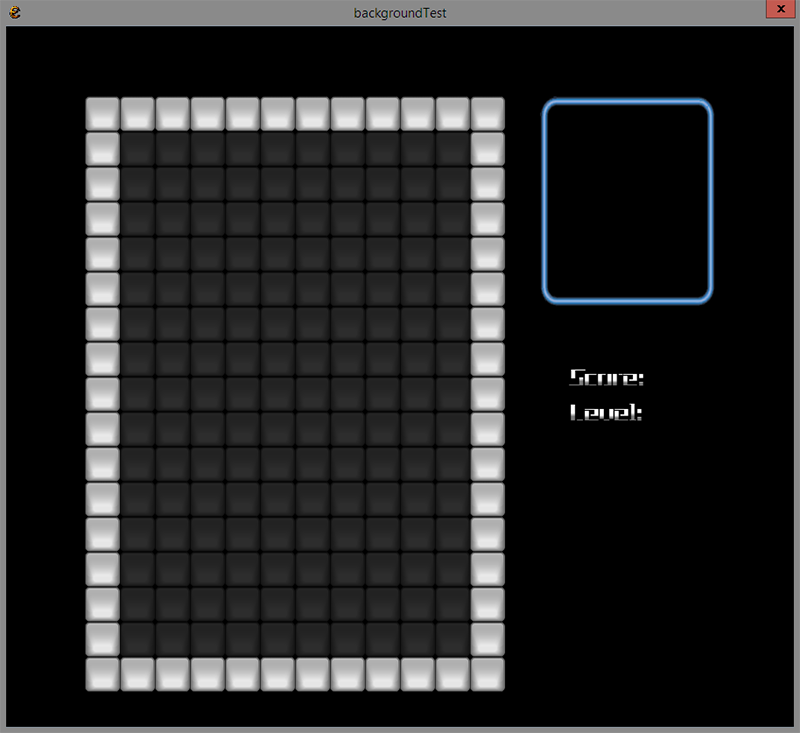
\includegraphics[width=0.6\linewidth]{../images/tetris_background.png}
\caption[]{De tetris achtergrond}
\label{fig:tetris_background}
\end{figure}

Om het speelveld te tekenen gebruiken we squares. Dat had ook een afbeelding kunnen zijn, maar zo houden we de interface conform met het spel. Daarnaast heb je een \eeClass{Rect} nodig om een afbeelding te tonen op de plaats waar het volgende blok verschijnt. Tot slot moeten we de positie weten waar we de score en het level tonen.

\begin{code}
class background
{
   Mems<square> squares;
   Rect blockRect;
   Vec2 scorePos;
   Vec2 levelPos;
   
   void create()
   {
   }
   
   void draw()
   {
   }
}

background Background;
\end{code}

In je testprogramma kan je nu al de twee functies van deze class tonen. Daarnaast voeg je de volgende regel toe aan de functie \eeFunc{InitPre}:

\begin{code}
D.mode(WINDOW_WIDTH, WINDOW_HEIGHT);
\end{code}

Deze regel zorgt ervoor dat het window van de applicatie de grootte krijgt die we bij de definitie van de constanten ingaven. Bij de vorige testprogramma's was dat nog niet nodig, maar bij de achtergrond willen we wel zien wat het uiteindelijke resultaat is.

\subsection{Speelveld}

Zoals je weet is het speelveld een grid. Omdat we ook een `muur' rond het speelveld tekenen, beginnen we niet op positie 0 maar op positie -1 met het toevoegen van squares. De squares in het veld zelf geven we het type \eeFunc{BT\_BACKGROUND}. De muren krijgen het type \eeFunc{BT\_WALL}. Daardoor zullen ze in een andere kleur op het scherm gezet worden.

De code om de nodige squares toe te voegen krijg je kado. Eigenlijk is ze niet zo moeilijk, maar wel als je er voor het eerst aan moet beginnen. Lees deze code dus goed en vraag uitleg als je niet begrijpt hoe ze werkt. Daarna voeg je ze toe aan de functie \eeFunc{create}.

\begin{code}
for(int x = -1; x <= SQUARES_PER_ROW; x++)
{
	 for(int y = -1; y <= ROWS; y++)
	 {
			if(x == -1 || y == -1 || x == SQUARES_PER_ROW || y == ROWS)
			{
				 squares.New().create(VecI2(x, y), BT_WALL);
			} else
			{
				 squares.New().create(VecI2(x, y), BT_BACKGROUND);
			}
	 }
}
\end{code}

In de draw functie begin je met het scherm zwart te maken. Daarna toon je alle elementen van de container squares. Test je programma en controleer het resultaat.

\subsection{Next Block}
Op de plaats waar het volgende blok verschijnt plaatsen we een afbeelding. We hebben daar al een constante \eeFunc{WAITPOS} voor gemaakt. Maar dat is een positie in de grid. We moeten die dus steeds vermenigvuldigen met de grootte van een square (de constante \eeFunc{SQUARE\_SIZE}). Daar komt ook nog bij dat we pas mogen tellen vanaf het speelveld, en dat is de constante \eeFunc{GAMEAREA}.

Om te beginnen kunnen we daarom de volgende positie berekenen:

\begin{code}
Vec2 blockPos = GAMEAREA + (WAITPOS * SQUARE_SIZE);
\end{code}

Maar zoals je weet heb je voor een rechthoek een minimum en een maximum nodig. Als minimum trekken we van de gevonden positie twee squares af. Het zou logisch zijn om dan voor de maximum positie twee squares extra te rekenen. Later zal je zien dat dat er visueel minder goed uit ziet, maar dat kan je dan zelf aanpassen. De laatste regel gebruikt de twee nieuwe waarden om de eigenlijke rechthoek in te stellen.

\begin{code}
Vec2 min = blockPos - (2 * SQUARE_SIZE);
Vec2 max = blockPos + (2 * SQUARE_SIZE);
blockRect.set(min, max);
\end{code}

Voeg nu aan de functie \eeFunc{draw} code toe om de afbeelding `tetris\_score' te tekenen via de rechthoek die je net berekende.

\subsection{Tekst}
Je hebt nog twee posities nodig: \eeFunc{scorePos} en \eeFunc{levelPos}. Voor de positie van de score neem je blockPos als uitgangspunt. Van de vertikale waarde trek je vier maal de \eeFunc{SQUARE\_SIZE} af. Voor de level positie vertrek je van de gevonden positie voor de score, maar trekt van de vertikale waarde nog eens \'e\'en square af.

Als je dat in orde hebt kan je te score op het scherm tekenen. Voorlopig zet je daar enkel een tekst. De echte score voegen we later toe. Er is trouwens ook een speciaal font voorzien om in dit spel te gebruiken. Dat is het bestand gui $\Rightarrow$ tetrisFont $\Rightarrow$ tetris Style. Als je niet meer weet hoe je het uitzicht van een tekst moet aanpassen, kan je dat nakijken in hoofstuk \ref{chapter:tekstopmaak}.

Test uiteindelijk weer je programma.

\section{Het geluid}
De volgende class die we maken is \eeClass{soundManager}. Die is behoorlijk eenvoudig en je kan die zelf uitwerken. Er zijn geen create functies nodig, enkel functies die een bepaald geluid afspelen. Je voorziet de volgende functies:

\begin{enumerate}
  \item startMusic: start de soundtrack in een loop.
	\item blip: speelt het `blip' geluid.
	\item score: speelt het `rowdone' geluid.
	\item win: speelt het `won' geluid.
	\item lost: speelt het `lost' geluid.
	\item rotate: speelt het `rotate' geluid.
	\item moveDown: speelt het `down' geluid.
\end{enumerate}

Ook van deze class heb je maar \'e\'en object nodig, dus je maakt onder je class het object \eeClass{SoundManager}. Daarna kan je een eenvoudig testprogramma maken waarin je door op toetsen te drukken deze geluiden afspeelt. Zorg ervoor dat alle geluiden ongeveer even luid klinken. Indien nodig pas je in je class het volume van bepaalde geluiden aan.
